\documentclass{article}
\usepackage{graphicx}
\usepackage[margin=1in]{geometry}
\usepackage{subcaption}
\usepackage{csvsimple}
\usepackage{booktabs}
\usepackage{pgfplotstable, colortbl} %for making tables from csv files
%\pgfplotset{compat=1.16}
\usepackage{longtable} %to fix my long table
\usepackage{tabu} % if you want - to fix a wide table

\begin{document}

\title{Simulation Write Up{}}
\author{Amy Solman}

\maketitle

\section{Aims}
To test the hypothesis that the predictions made by Chisholm’s model are significantly statistically similar to the results of the island simulation. \bigskip

\noindent To test the hypothesis that, as island area increases, it transitions from a niche-structured regime, to a colonisation-extinction balance regime. 

\section{Methods}

\subsection{Simulation Design}

\subsubsection{Overview}
This simulation is designed to mimic the process of island colonisation from a metacommunity. The colonisation process is constrained by migration rate and each island is characterised by number of niches and the size of each niche. The output of the simulation is the final community in each niche of each island, as well as a timeseries of species richness. 

\subsubsection{Metacommunity}
A metacommunity is generated at the beginning of the simulation using \textit{coalescence\_test} function, partially modified from a script provided by Dr James Rosindell. The function takes the input parameters: metacommunity size(\textit{J\_meta} = 50 000) and speciation rate (\textit{nu} = 0.001). Each run of the function produces 20 niche communities, each of size \textit{J\_meta}/20.  \bigskip

\noindent The function initialises a vector (\textit{lineages}) of length = \textit{J\_meta}/20 = \textit{niche\_size} with 1 as every value. An empty vector (\textit{abundances}) is initialised. The value of \textit{niche\_size} is given to \textit{N}. \textit{Theta} is calculated as \textit{nu*(niche\_size-1)/(1-nu)}. Then, while \textit{N $>$ 1}, a vector (\textit{linvect}) is created with values 1:length(\textit{niche\_size}). A random sample of \textit{linvect} is made (\textit{j}). A random decimal number is selected between 0 and 1 (\textit{randnum}). If \textit{rannum} is less than \textit{theta/(theta+N-1)}, then the value at \textit{lineages[j]} is appended to \textit{abundances}. Else, another random number (\textit{i}) is sampled from \textit{linvect}, excluding the last number selected. The values at \textit{lineages[i]} and \textit{lineages[j]} are summed and take the position of \textit{lineages[i]}. \textit{lineages[j]} is then removed from \textit{lineages}, so the vector is one value shorter. The value of \textit{N} is also decreased by 1. This repeats until \textit{N} = 1. The remaining value in the \textit{lineages} vector is added to \textit{abundances} and the function outputs a vector of simulated species abundances.\bigskip

\noindent At the end of the \textit{coalescence\_test} function, each of the 20 niches is assigned a letter type from A to T. A list of niche communities in the metacommunity is returned. It was chosen to generate no more than 20 niches within the metacommunity, because the simulation would not go beyond modelling 20 niches on an island. Any additional niches generated for the metacommunity would go unused. \bigskip

\noindent The \textit{coalescence\_test} function is incorporated into a second function (\textit{metacommunity}), that generates a vector of individuals from each niche abundance vector. For example, Niche A \textit{abundances}(5,4,2,2,1,1) would generate a community \textit{meta\$A}(1,1,1,1,1,2,2,2,2,3,3,4,4,5,6) where each unique number value represents a unique species.%\bigskip     

\subsubsection{Parameters}
The variable parameters of the simulation are: migration rate (range: 0.003-0.06), number of niches (range: 1-20), size of niches (range:1-20). Each unit of space was assumed to host one individual, therefore, number of niches x size of niches = area = size of island population. There are a total of 8000 condition combinations applied during the simulation (20 migration rates, 20 number of niches, 20 size of niches). 

\subsubsection{Simulation Logic}
At timestep \textit{i} an island is selected. The first niche on that island becomes the focal niche. An individual within that niche is chosen to die. With probability \textit{m} (migration rate), the dead individual is replaced with a randomly chosen propagule from the same niche type in the metacommunity (e.g. from metacommunity niche A to island niche A). With probability 1 - \textit{m}, the dead individual is replaced with a local propagule from the same niche. The simulation then moves to the next niche on that island. When all niches have been simulated for timestep \textit{i}, the simulation moves to the next island. When all islands have been simulated for timestep \textit{i}, the simulation moves to the next timestep \textit{i + 1}, and returns to the first island (Figure 1). The species richness for each niche is calculated, totaled across all niches for each island and stored at every 5000 timesteps.

\bigskip
 
 \begin{figure}[h!]
\centering
  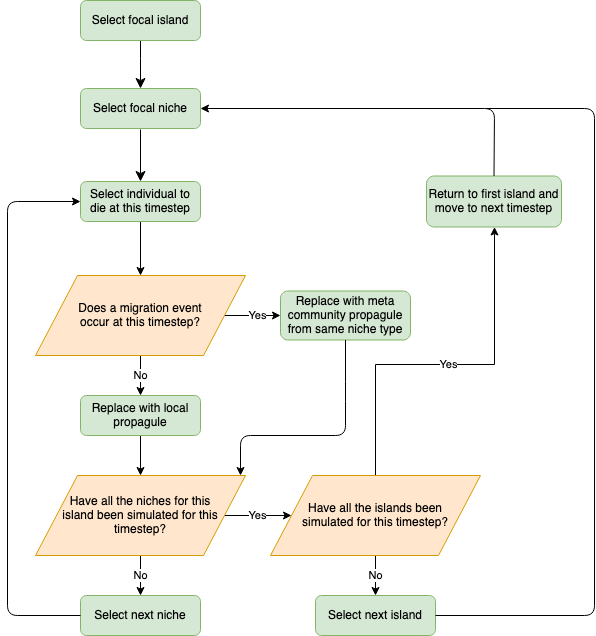
\includegraphics[scale=0.4]{../../../Other/neutral_flowchart2.png}
  \caption{Flowchart of simulation design}
  \label{fig:Flowchart}
\end{figure}


\subsubsection{High Performance Computing}
The metacommunity and simulation code are contained in \textit{ClusterSim.R}. \textit{ClusterSim.R} functions are sourced by \textit{ClusterCode.R} and given the input parameters: \textit{J\_meta} = 50000, \textit{nu} = 0.001, \textit{num\_m\_rates} = 20, \textit{max\_k\_num} = 20, \textit{max\_k\_size} = 20, \textit{wall\_time} = 1380, \textit{output\_file\_name} = output\_file\_name (where each simulation is given a unique file name "simulation\_timeseries\_\textit{i}". \textit{ClusterRun.sh} is used to run on the cluster, with a time limit of 24:00:00. \textit{wall\_time} is given as 1380 minutes (23 hours) within the function, to ensure all simulations are completed before the cluster run ends. 100 parallel simulation were run on the Imperial College London High Performance Computing service. This generated a total of 800000 islands, simulated for $>$ 30000 timesteps.   

\subsection{Data Preparation and Timeseries Plots}
The 100 simulation results were imported into \textit{DataPrep.R}. The data from each island was isolated and configured into a data frame with simulation number, migration rate, area, number of niches and number of species (\textit{SimModelFitData.csv}). A second data frame was generated for timeseries plotting, with simulation number, island number, migration rate, timestep and species richness timeseries for each island (\textit{SimTimeseriesPlotData.csv}).\bigskip

\noindent To ensure the simulation had run long enough for each island to reach dynamic equilibrium the species richness timeseries of simulations 25, 50 and 75 were plotted(\textit{TimeseriesPlot.R})(Figure 2).

\subsection{Analysis}\bigskip

\begin{verbatim}
chisholm_model <- function(area, theta, m0, K) {
  rho = 1
  K = K
  Js = area*rho
  J_stars = Js/K
  ms = m0/sqrt(area)
  gamma_stars = J_stars*ms/(1-ms)
  return(theta*(digamma(theta/K+gamma_stars*
  (digamma(gamma_stars+J_stars)-digamma(gamma_stars)))-digamma(theta/K)))
}
\end{verbatim}

\noindent An analysis script (\textit{Analysis.R}) imported the prepared data (\textit{SimModelFitData.csv}) for each island across all simulations (800000 islands). Model estimated species richnesses were generated by giving the island parameters (\textit{m0 = m*sqrt(area)}) and an estimated \textit{theta} (\textit{theta = 2*(niche\_size*K)*nu}, where \textit{niche\_size * K} = size of each niche in the metacommunity from which immigration events can occur times by the number of niches contributing to the island community i.e. number of niches on the island). The results of the simulation and those estimated by the \textit{chisholm\_function} (above) were bound together in a data frame. Mean species richness results for each combination of island area, migration rate and number of niches across all 100 simulations was calculated and stored.
  
\subsubsection{Within Simulation Analysis}

\paragraph {Repeatability} 
The repeatability of the simulation was assessed by running a linear model of species richness, with simulation number as independent variable. The repeatability statistic was calculated by running an ANOVA on the model and finding the among simulation and within simulation variabilities.

\paragraph{Normality}
The normality of the simulation data was assess by generating histograms of island species richnesses. It was necessary to check the normality of the data as linear regression assumes normality.

\paragraph{Collinearity}
The collinearity of the simulation independent variables was assessed by using the R base function pairs() to produce a scatterplot of matrices. This allowed for visual inspection of the relationships between migration rate, island area and number of niches. It is important to assess the collinearity of covariates because it can inflate variation. Large amounts of collinearity cause covariates to have larger standard errors and it becomes less likely to detect a significant result. The Variance Inflation Factor (VIF) was calculated to ensure the collinearity between number of niches and island area was within acceptable limits for this analysis. 

\paragraph{Linear Regression}
Linear regression was carried out to investigate whether there was a statistically significant relationship between the dependent variable (species richness) and independent variables (area and niches). Migration rate was excluded from the linear regression analysis as previous collinearity statistics indicated it was not significant in predicting species richness (this is later confirmed in multivariate analysis). The mean species richness for each unique set of parameters across all 100 simulations was calculated. Area and niche variables were then z-transformed so that they could better meet the assumptions of a linear model and the intercept statistic would then give the mean of the dependent sample. Histograms of the residuals of each linear model were generated to check for homogeneity of the variances, to validate the assumptions of the regression analyses. The models were validated by visual inspection of the distribution of the residuals. 

\paragraph{Multivariate Analysis}
Multivariate analysis of the mean simulation data, including number of niches, island area and migration rate was performed to investigate to what extent the three independent variables predicted species richness. A second multivariate analysis was carried out, excluding migration rate. Model results were plotted to check the distribution of the residuals.

\subsubsection{Simulation/Model Comparison}

\paragraph{Outliers}
Both the simulation dataset and model estimated species richnesses were checked for outliers using boxplots. This ensured analysis was not skewed by anomalous results.

\paragraph{Mean, range, variance, standard deviation and standard error}
The mean, range, variance, standard deviation and standard error of the simulation and the \textit{chisholm\_function} estimated species richnesses were calculated. 

\paragraph{Paired-sample t-Test}
A paired-sample t-test was used to assess whether the mean difference between the simulation results and \textit{chisholm\_function} estimates was zero. A paired-sample t-test was used because both sets of species richness data were calculated from the same set of parameters (migration rate, number of niches, island area) and were directly comparable across pairs. 

\paragraph{Non-Linear Least Squares Fitting}
The model was also fit to the data using non-linear least squares (NLLS) fitting. The 800000 simulated islands were subset by migration rate and number of niches (400 combinations). For each of the 400 datasets, the mean species richness for each island area was calculated. The \textit{chisholm\_function} was then fit to the mean species richness dataset for each unique combination of parameters using NLLS fitting.

\subsection{Repeat Analysis with Reducing Data Set}

\begin{table}[ht]
\caption{Reducing dataset to smaller islands}
\centering
    \begin{tabular}{l|l}%
    \bfseries Max Island Size & \bfseries Num. Islands% specify table head
    \csvreader[head to column names]{../../../Results/Simulation2/DividedDF.csv}{}% use head of csv as column names
    {\\\hline\csvcoli&\csvcolii}% specify your coloumns here
    \end{tabular}
    \end{table}

\noindent Within simulation analysis was repeated 20 times whilst reducing the dataset by limiting maximum island area (Table 1). This allowed for comparative multivariate analysis, to ascertain if the relative significance of the independent parameters changed as island area decreased.\bigskip

\noindent All data preparation, analysis and plotting were carried out using R 3.6.0 and Python 2.7.16.


\section{Results}

\begin{figure}[!h]
\centering
  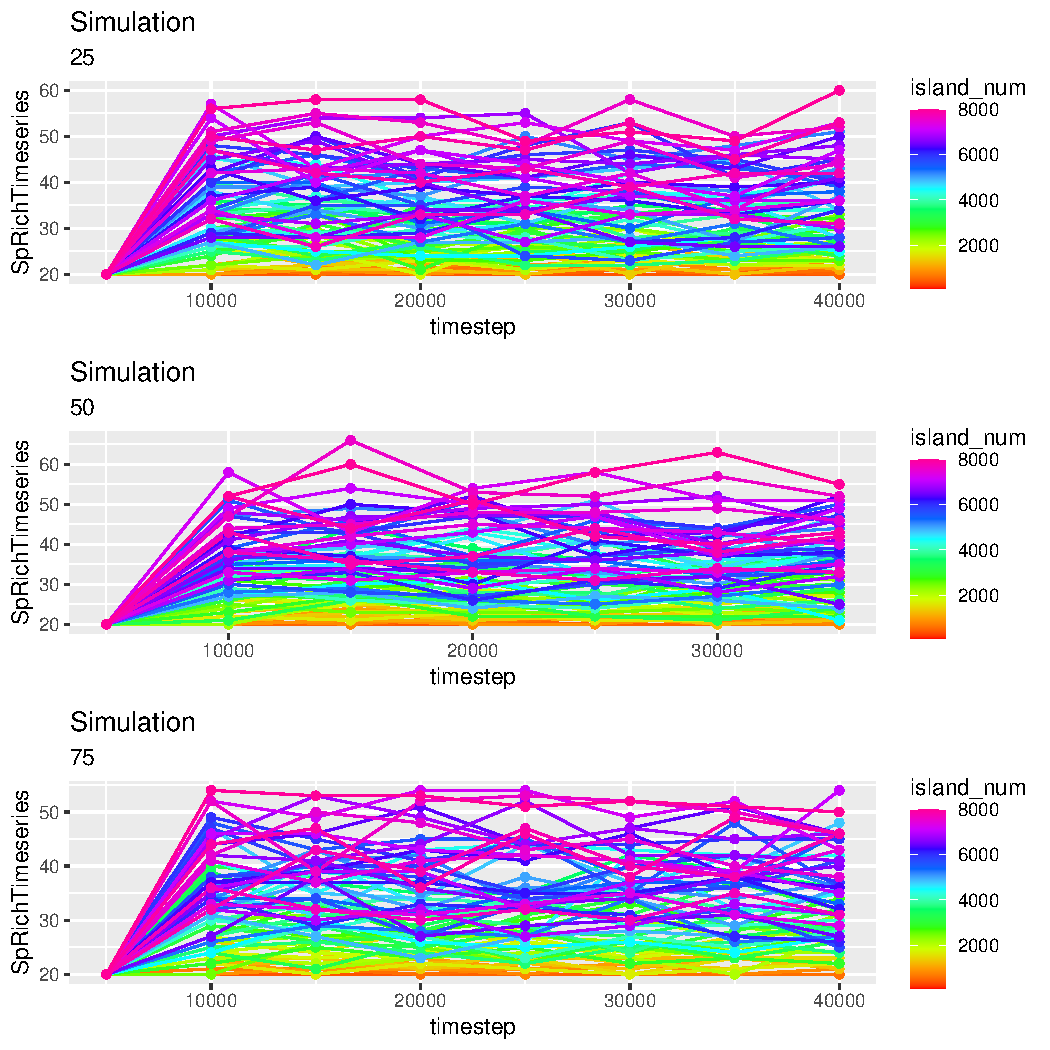
\includegraphics[scale=0.5]{../../../Results/Simulation2/TimeseriesPlot.pdf}
  \caption{Timeseries plot of three simulations}
  \label{fig:Timeseries plot}
\end{figure}

\subsection{Within Simulation Results}

\subsubsection{Timeseries}
3 of 100 simulation were selected and plotted as a timeseries (Figure 2). From this plot it was determined that the islands reached dynamic equilibrium at approximately 15000 timesteps. The simulation had run for enough time to reach dynamic equilibrium.

\subsubsection{Repeatability} %Not entirely sure on repeatability, is this right?
The mean sum of squared variance among simulations was 670.9 (Vg). The mean sum of squared variance within simulations was 109.5 (Vr). The repeatability of the simulations was calculated as Vg / (Vg + Vr)  = 0.86. 86\% of the variation in species richness is determined by between-simulation differences. The simulations are giving fairly consistent values of species richness, indicating the method is robust. 

\subsubsection{Collinearity}

\begin{figure}[!h]
  \centering
  \begin{subfigure}[b]{0.4\linewidth}
    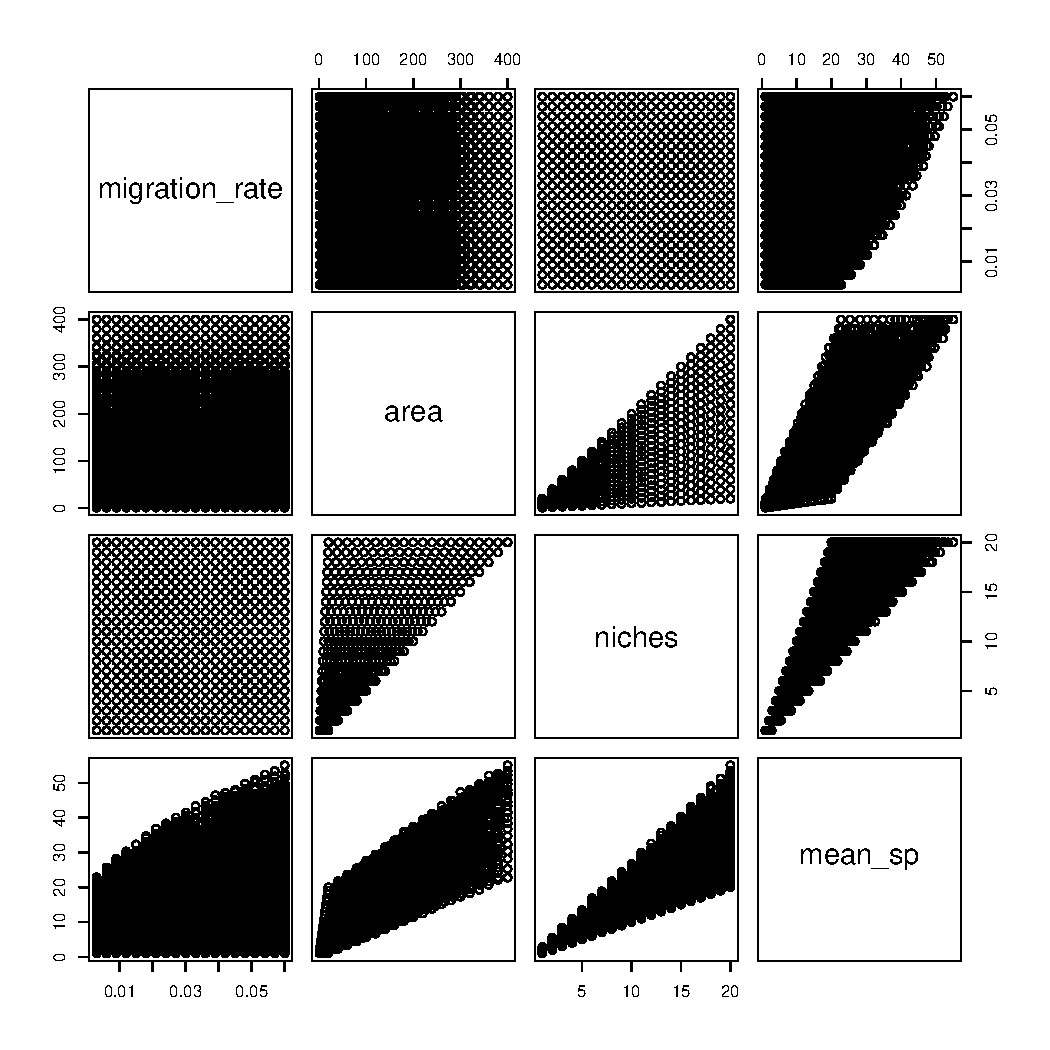
\includegraphics[width=\linewidth]{../../../Results/Simulation2/CollinearityPlot_1.pdf}
    \caption{maxArea = 400 units}
  \end{subfigure}
  \begin{subfigure}[b]{0.4\linewidth}
    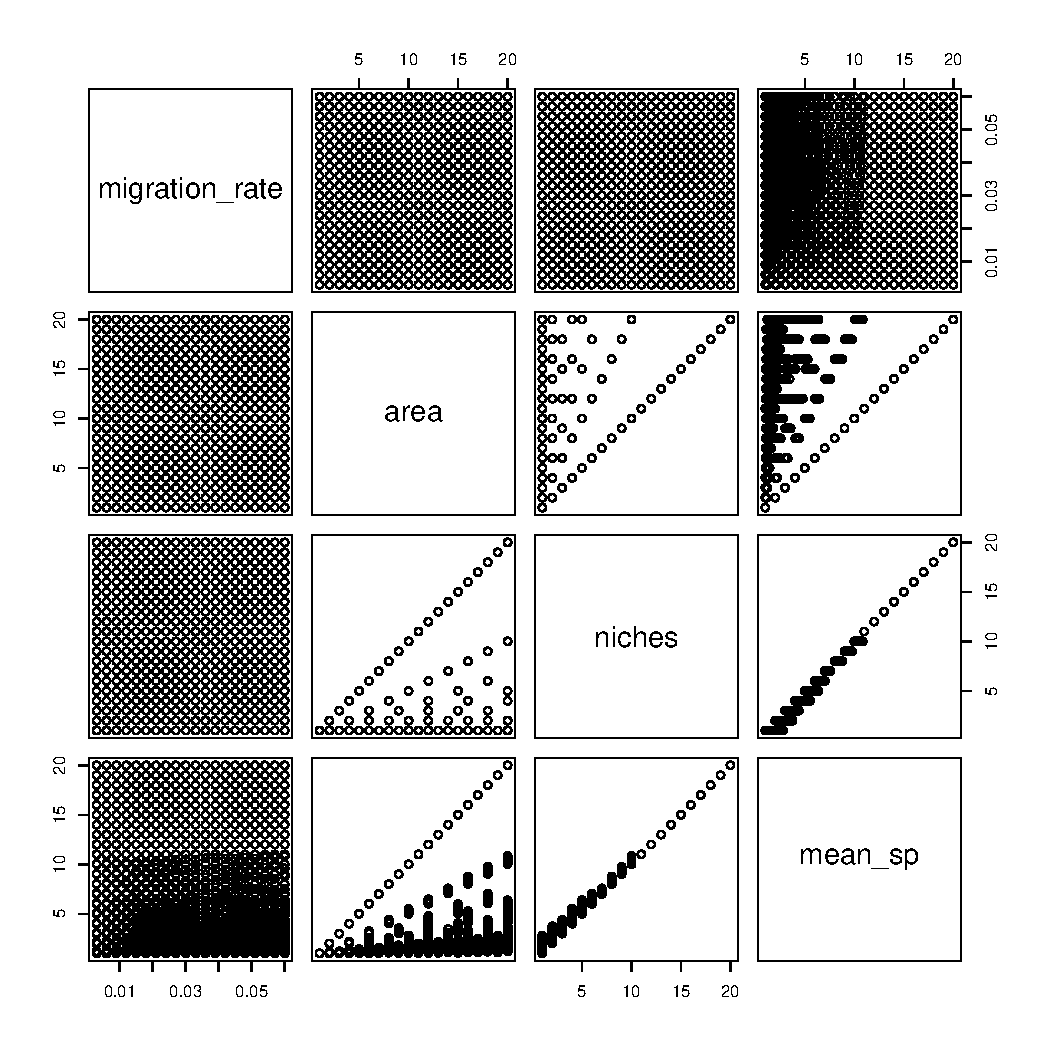
\includegraphics[width=\linewidth]{../../../Results/Simulation2/CollinearityPlot_20.pdf}
    \caption{maxArea = 20 units}
  \end{subfigure}
  \caption{Collinearity plots for full data set (a) and reduced data set (b)}
  \label{fig:Collinearity}
\end{figure}\bigskip

\noindent The collinearity statistic for migration rate and area, as well as migration rate and niches was 0. A lack of collinearity between migration rate and the other covariates is to be expected as they are not logically linked in the simulation, nor would they be in a real-world scenario. Area and niches had a collinearity score of 0.659. The VIF score for collinearity between niches and area was 1.77. The standard errors of number of niches are therefore inflated by $\sqrt{1.77}$ = 1.33, which is within an acceptable range. \bigskip

\noindent The collinearity statistic for migration rate and area, as well as migration rate and niches in the most reduced dataset was 0. Area and niches had a collinearity score of 0.355 and VIF score of 1.14. The standard errors of number of niches are therefore 1.07. This is less than that of the whole dataset and therefore in an acceptable range. Visual inspection of pairs plots (Figure 3) supported the collinearity statistics. 

\subsubsection{Linear Regression Analysis}

\begin{table}[h!]
\centering
\caption{Linear regression results for z-transformed area and niches}
\pgfplotstabletypeset[
    col sep=comma,
    ignore chars={",_}, %get rid of quote marks around my text and ignore underscores
    string type,
    every head row/.style={%
        before row={\hline
           % \multicolumn{2}{c}{incase you wanted a title above the column headers} & \\
        },
        after row=\hline
    },
    every last row/.style={after row=\hline},
    columns/maxArea/.style={column name=maxArea, column type=c},
    columns/Coefficients/.style={column name=Coefficients, column type=c},
    columns/Estimate/.style={column name=Estimate, column type=c},
    columns/standarderror/.style={column name=StandardError, column type=c},
    columns/tvalue/.style={column name=tValue, column type=c},
    columns/pvalue/.style={column name=pValue, column type=l}, %problem with less than sign
    columns/rsquared/.style={column name=rSquared, column type=c},
    columns/variate/.style={column name=Variate, column type=l},
    ]{../../../Results/Simulation2/LMMaxMin.csv}
   \end{table}\bigskip

\noindent The linear model results of species richness and z-transformed area gave an r-squared value of 0.73 with a p-value $<$ 0.001 (Table 2). This indicated that there was a positive, statistically significant relationship between area and species richness for the entire dataset. \bigskip

\begin{figure}[h!]
  \centering
  \begin{subfigure}[b]{0.4\linewidth}
    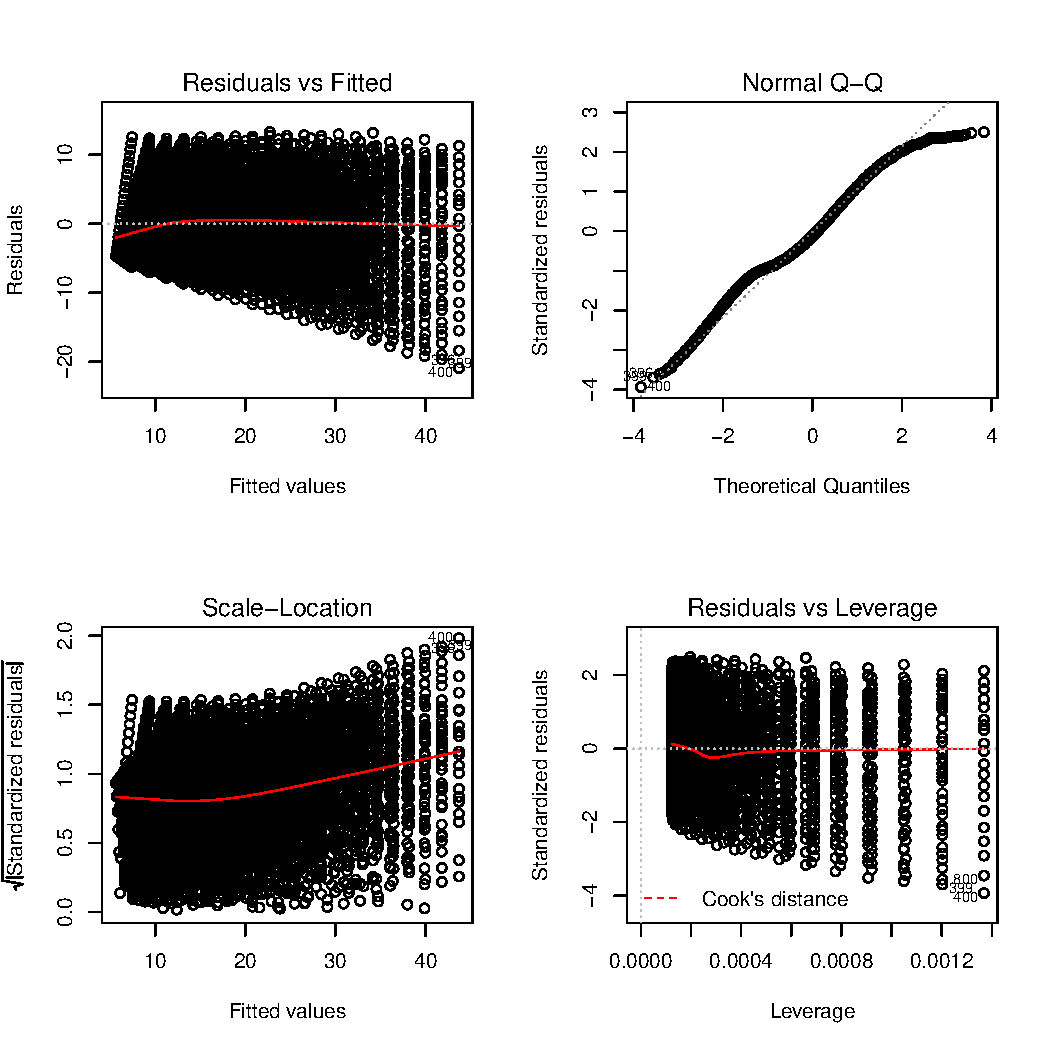
\includegraphics[width=\linewidth]{../../../Results/Simulation2/AreaSpeciesLmPlot_1.pdf}
    \caption{maxArea = 400 units}
  \end{subfigure}
  \begin{subfigure}[b]{0.4\linewidth}
    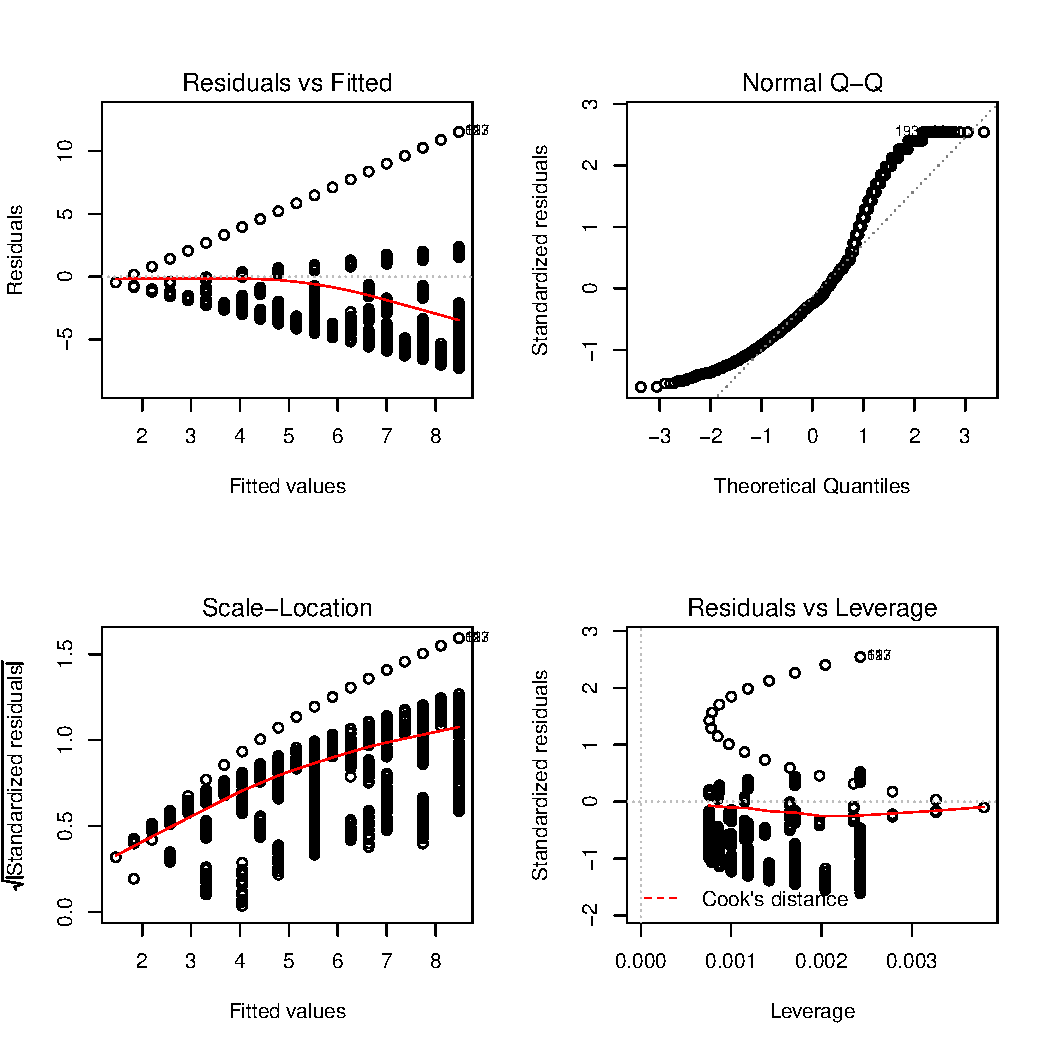
\includegraphics[width=\linewidth]{../../../Results/Simulation2/AreaSpeciesLmPlot_20.pdf}
    \caption{maxArea = 20 units}
  \end{subfigure}
  \caption{Model validation: Diagnostic plots of area and species richness linear models with full data set (a) and reduced data set (b)}
  \label{fig:Model validation area/species LM}
\end{figure}\bigskip

\begin{figure}[h!]
  \centering
  \begin{subfigure}[b]{0.4\linewidth}
    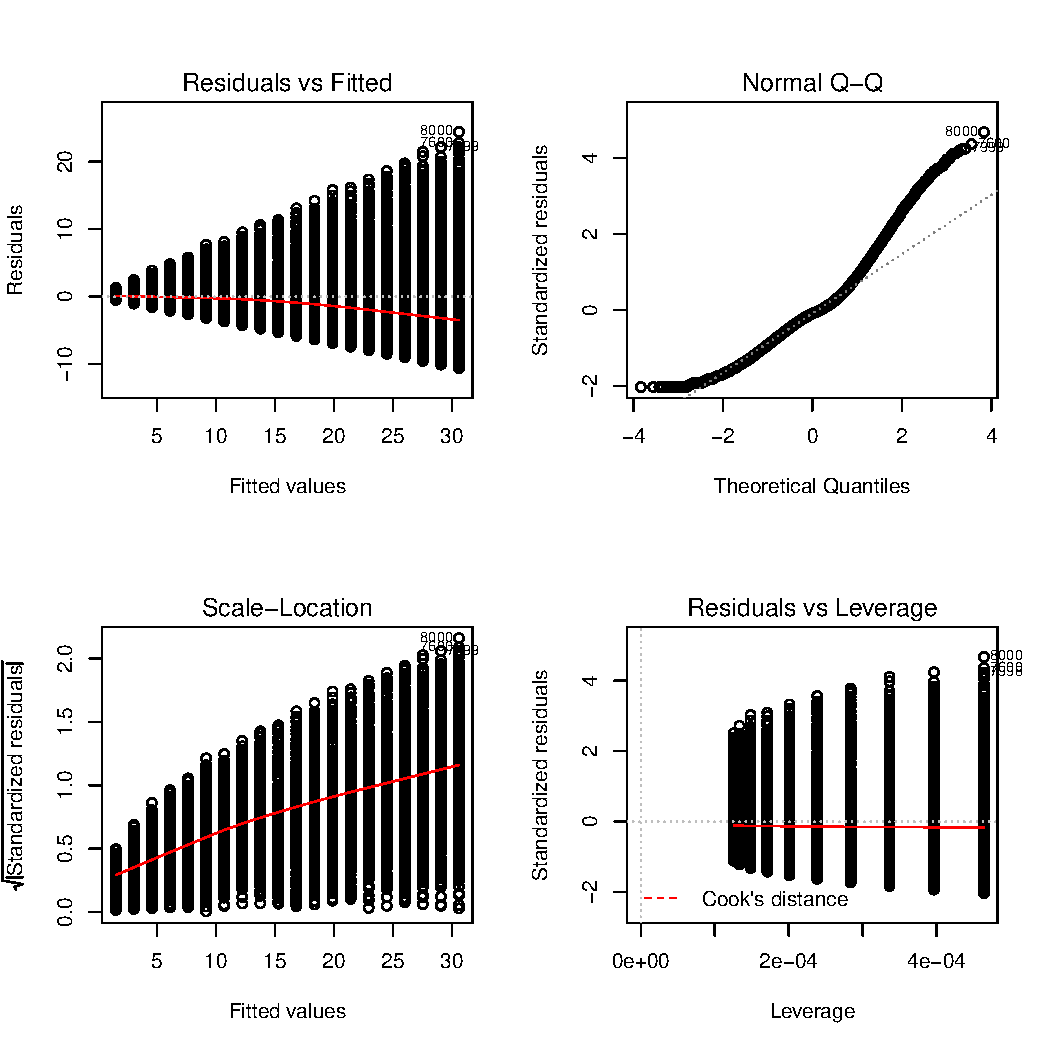
\includegraphics[width=\linewidth]{../../../Results/Simulation2/NicheSpeciesLmPlot_1.pdf}
    \caption{maxArea = 400 units}
  \end{subfigure}
  \begin{subfigure}[b]{0.4\linewidth}
    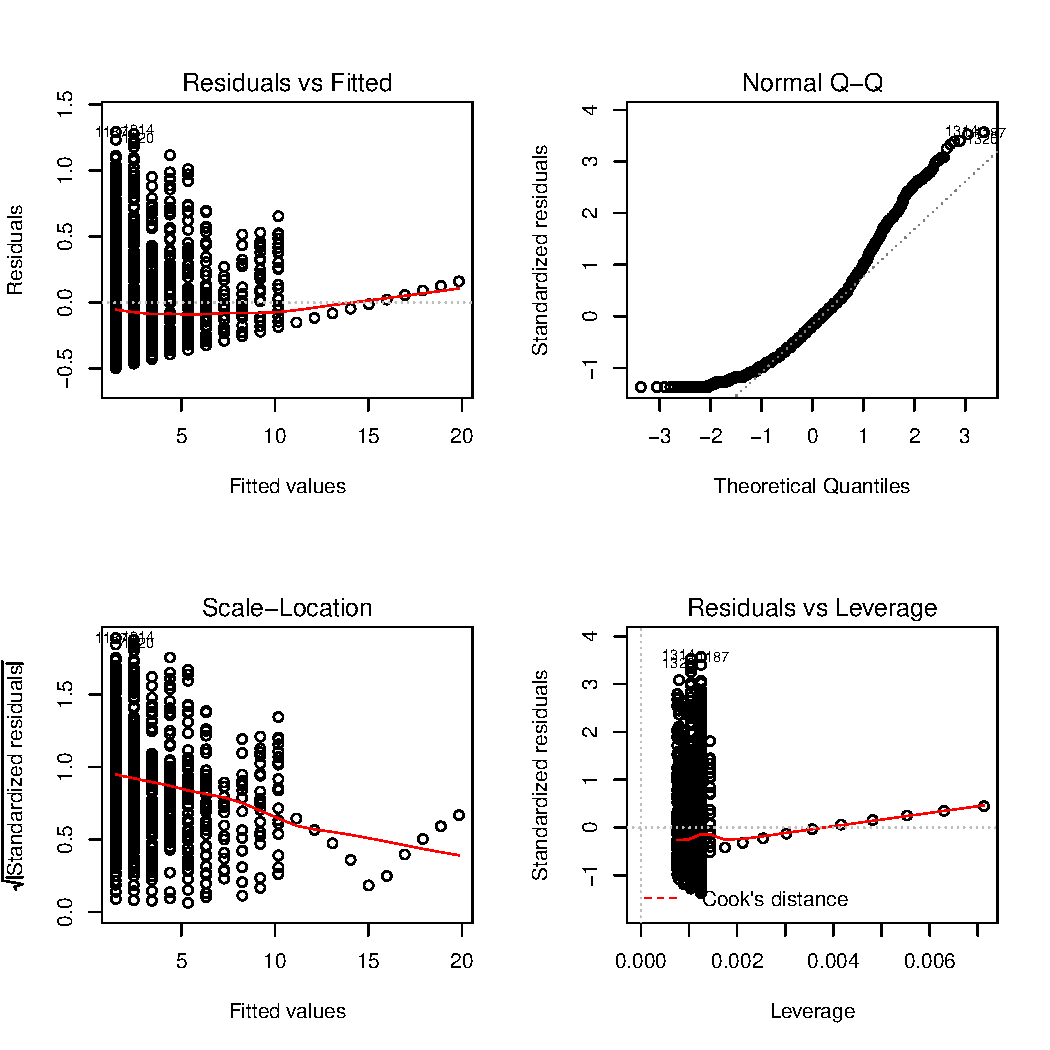
\includegraphics[width=\linewidth]{../../../Results/Simulation2/NicheSpeciesLmPlot_20.pdf}
    \caption{maxArea = 20 units}
  \end{subfigure}
  \caption{Model validation: Diagnostic plots of niche and species richness linear models with full data set (a) and reduced data set (b)}
  \label{fig:Model validation niche/species LM}
\end{figure}\bigskip

\noindent Visual inspection of residual vs fitted results for the entire dataset shows somewhat linear and constant variance (Figure 4 (a)). The normal Q-Q plot showing standardised residuals plotted against theoretical quantiles falls along a relatively straight line, with some deviation at the highest and lowest values. Diagnostics indicate the model works fairly well for the data.  \bigskip

\noindent The r-squared value for the area/species richness linear model reduced from 0.73 to 0.164 as maximum island area was reduce from 400 units to 20 units. This indicated that area had a weaker positive relationship with species richness as island area decreased (Figure 6). \bigskip

\noindent Visual inspection of the residual vs fitted plot for the most reduced dataset showed fairly linear but non-constant variance (Figure 4 (b)). Higher fitted values had a greater residual range than lower fitted values. The normal Q-Q plot deviated significantly at the highest values. Diagnostics indicate the model works somewhat well for the data at lower island areas. \bigskip

\noindent The linear model result of species richness and z-transformed niches gave an r-squared value of 0.741 with a p-value $<$ 0.001 (Table 2). This indicated that niches had a positive, statistically significant relationship with species richness. \bigskip

\noindent Visual inspection of the residual vs fitted plot for the entire dataset showed fairly linear but non-constant variance (Figure 5 (a)). Higher fitted values had a greater residual range than lower fitted values. The normal Q-Q plot deviated significantly at the highest values. Diagnostics indicate the model works somewhat well for the data. \bigskip

\noindent The r-squared value for niches/species richness linear model increased from 0.741 to 0.995 as maximum island area was reduced from 400 units to 20 units (Table 2). This indicated that number of niches had a stronger positive relationship with species richness as island area decreased (Figure 6). \bigskip

\noindent Visual inspection of the residual vs fitted plot for the most reduced dataset (Figure 5 (b)) showed weakly linear, non-constant variance. The normal Q-Q plot deviated significantly at the highest values.  Diagnostics indicate the model worked somewhat well for the reduced dataset. \bigskip

\begin{figure}[h!]
\centering
  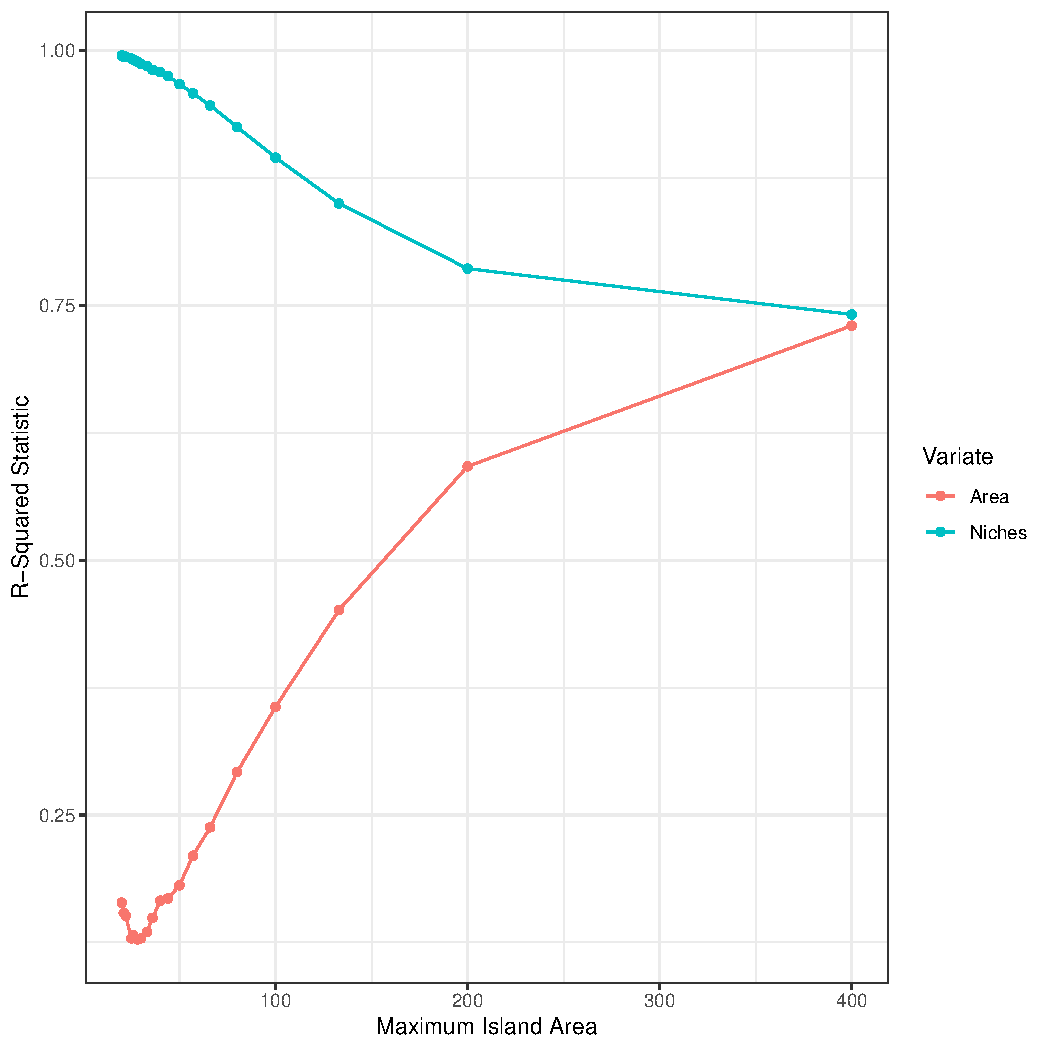
\includegraphics[scale=0.5]{../../../Results/Simulation2/LMRSquared.pdf}
  \caption{Change of R-squared statistic for number of niches and island area, with increasing island size}
  \label{fig:R-Squared statistic}
\end{figure}

\noindent Linear regression analysis for the reducing datasets indicated that at 400 units the islands transitioned from a niche dominated regime to an area dominated regime (Figure 6). 

\subsubsection{Multivariate Regression Analysis}

\begin{table}[h!]
\centering
\caption{Multiple regression analysis for z-transformed migration, area and niches}
\pgfplotstabletypeset[
    col sep=comma,
    ignore chars={",_}, %get rid of quote marks around my text and ignore underscores
    string type,
    every head row/.style={%
        before row={\hline
           % \multicolumn{2}{c}{incase you wanted a title above the column headers} & \\
        },
        after row=\hline
    },
    every last row/.style={after row=\hline},
    columns/maxArea/.style={column name=maxArea, column type=c},
    columns/Coefficients/.style={column name=Coefficients, column type=c},
    columns/Estimate/.style={column name=Estimate, column type=c},
    columns/standarderror/.style={column name=StandardError, column type=c},
    columns/tvalue/.style={column name=tValue, column type=c},
    columns/pvalue/.style={column name=pValue, column type=l}, %problem with less than sign
    columns/rsquared/.style={column name=rSquared, column type=c},
    columns/variate/.style={column name=Variate, column type=l},
    ]{../../../Results/Simulation2/MultiMaxMin.csv}
   \end{table}\bigskip
   
\noindent Multivariate analysis results for the whole dataset showed that the combined effects of number of niches, island area and migration rate gave an r-squared value of 0.95 (Table 3). The combined effects of niche and area gave an r-squared value of 0.887. This indicates that migration rate had a weak positive effect on species richness across the entire dataset.  \bigskip

\begin{figure}[h!]
  \centering
  \begin{subfigure}[b]{0.4\linewidth}
    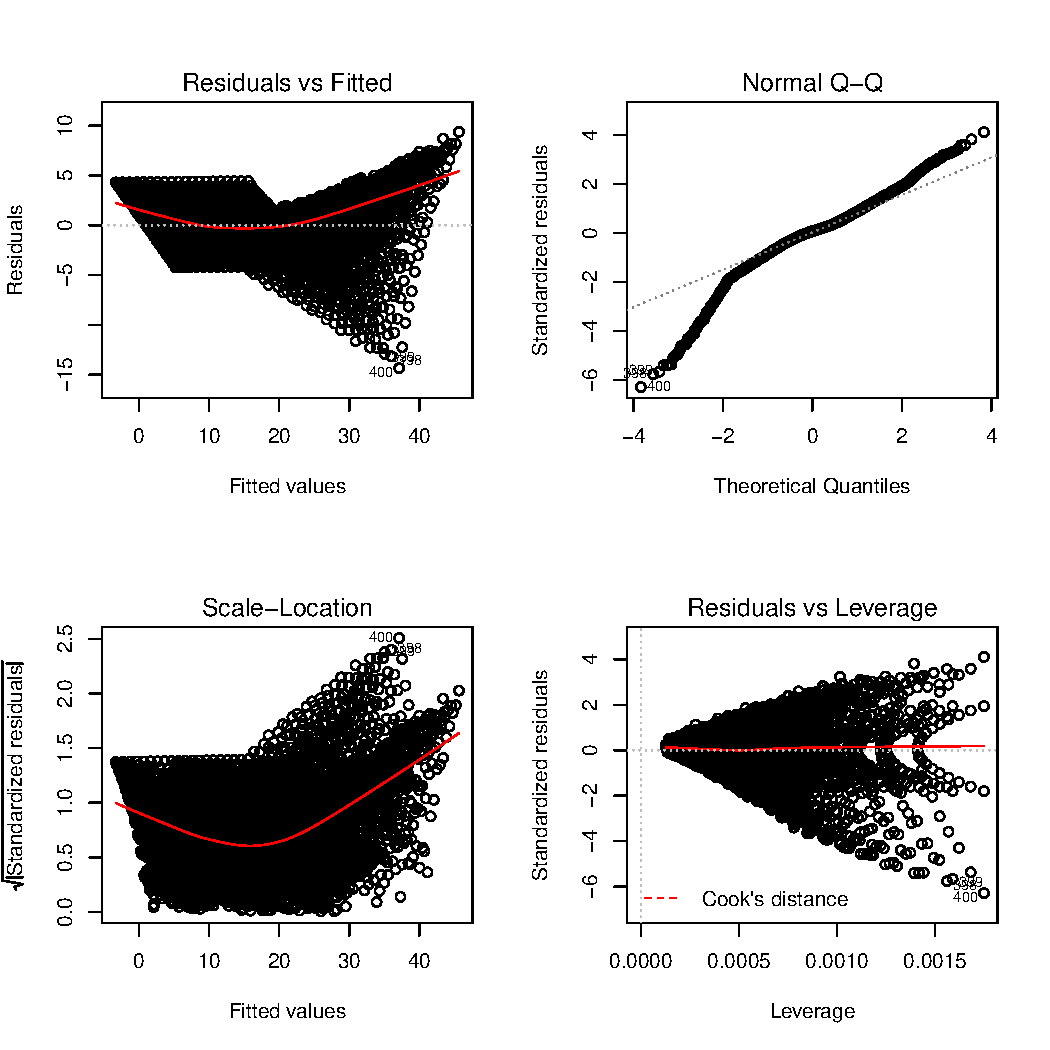
\includegraphics[width=\linewidth]{../../../Results/Simulation2/NicheAreaMigrationLmPlot_1.pdf}
    \caption{maxArea = 400 units}
  \end{subfigure}
  \begin{subfigure}[b]{0.4\linewidth}
    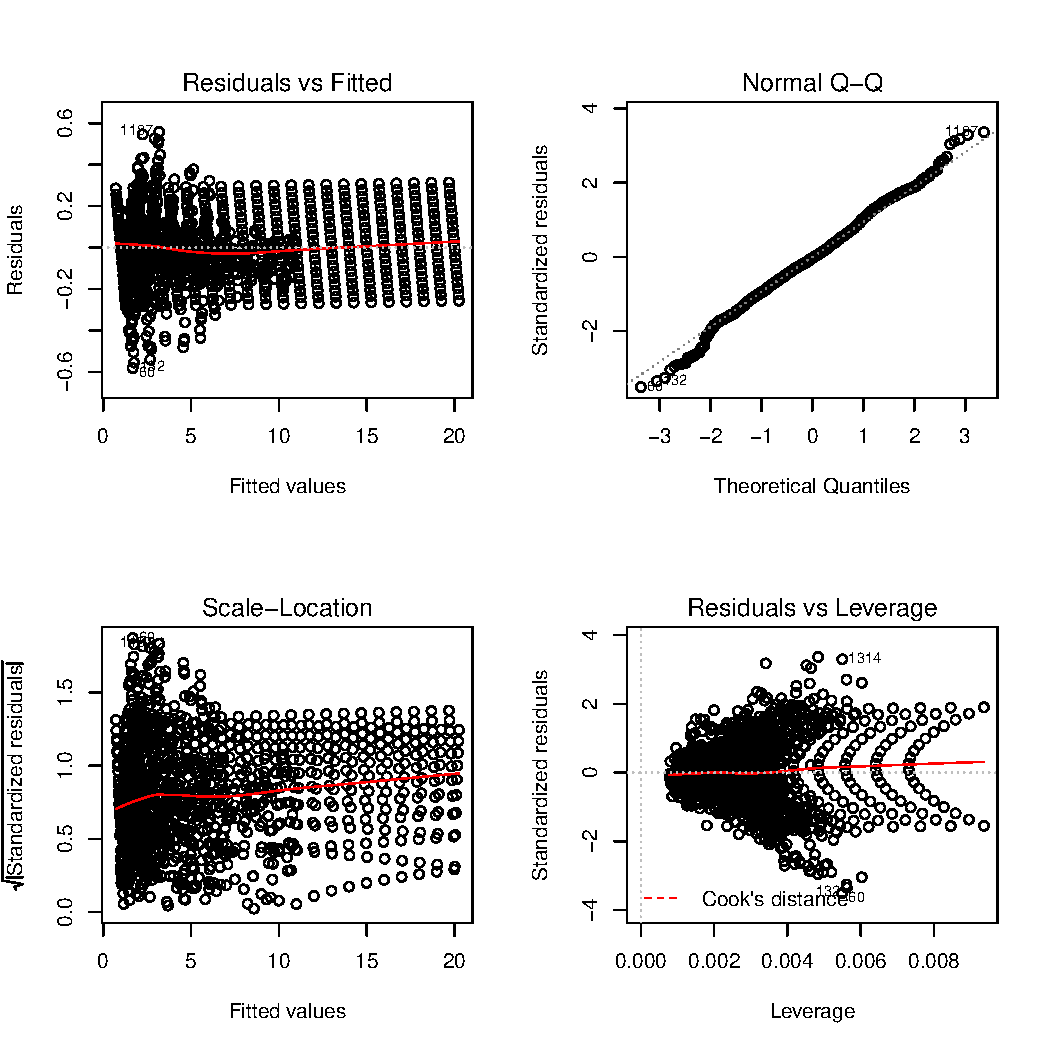
\includegraphics[width=\linewidth]{../../../Results/Simulation2/NicheAreaMigrationLmPlot_20.pdf}
    \caption{maxArea = 20 units}
  \end{subfigure}
  \caption{Model validation: Residuals plots of multivariate analysis of niche, area, migration and species richness with full data set (a) and reduced data set (b)}
  \label{fig:Model validation multivariate 1}
\end{figure}

\begin{figure}[h!]
  \centering
  \begin{subfigure}[b]{0.4\linewidth}
    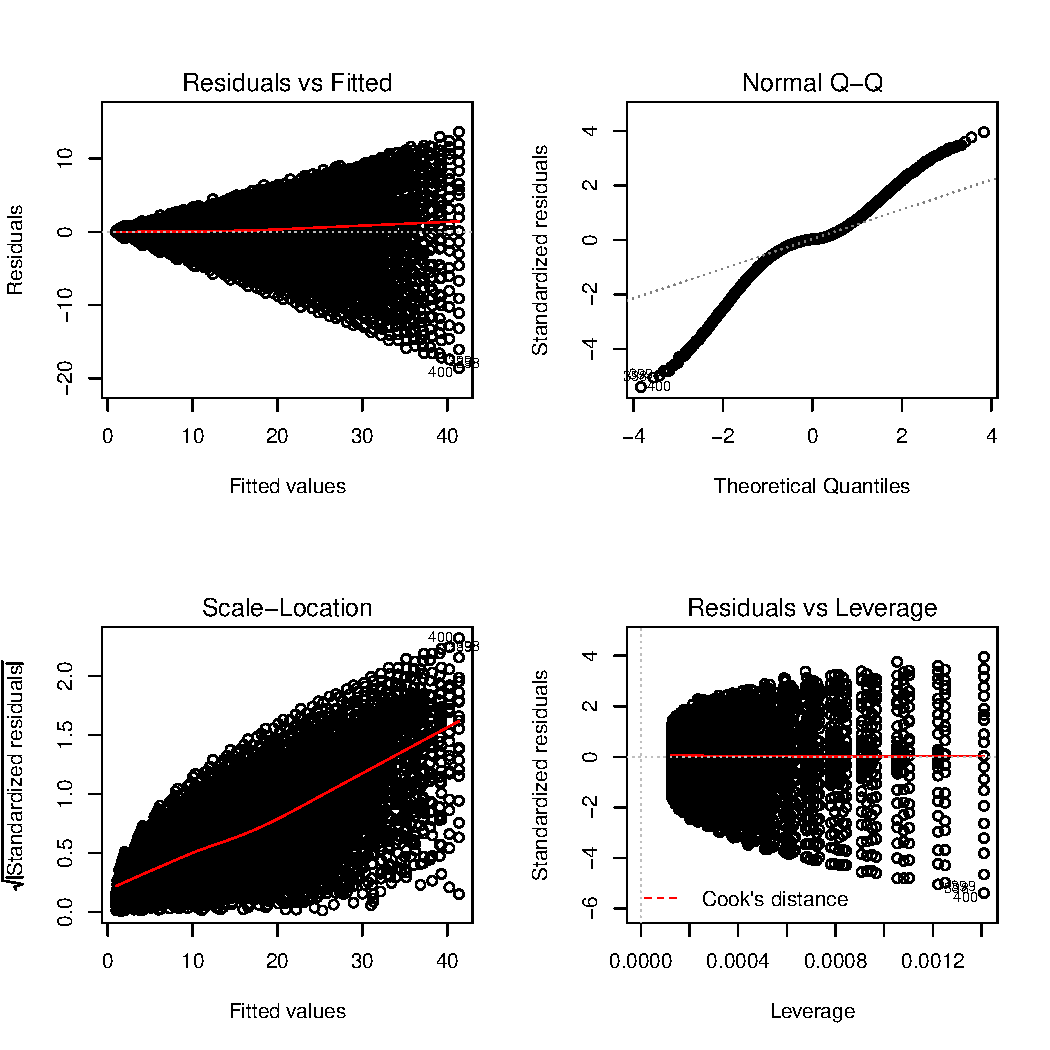
\includegraphics[width=\linewidth]{../../../Results/Simulation2/NicheAreaLmPlot_1.pdf}
    \caption{maxArea = 400 units}
  \end{subfigure}
  \begin{subfigure}[b]{0.4\linewidth}
    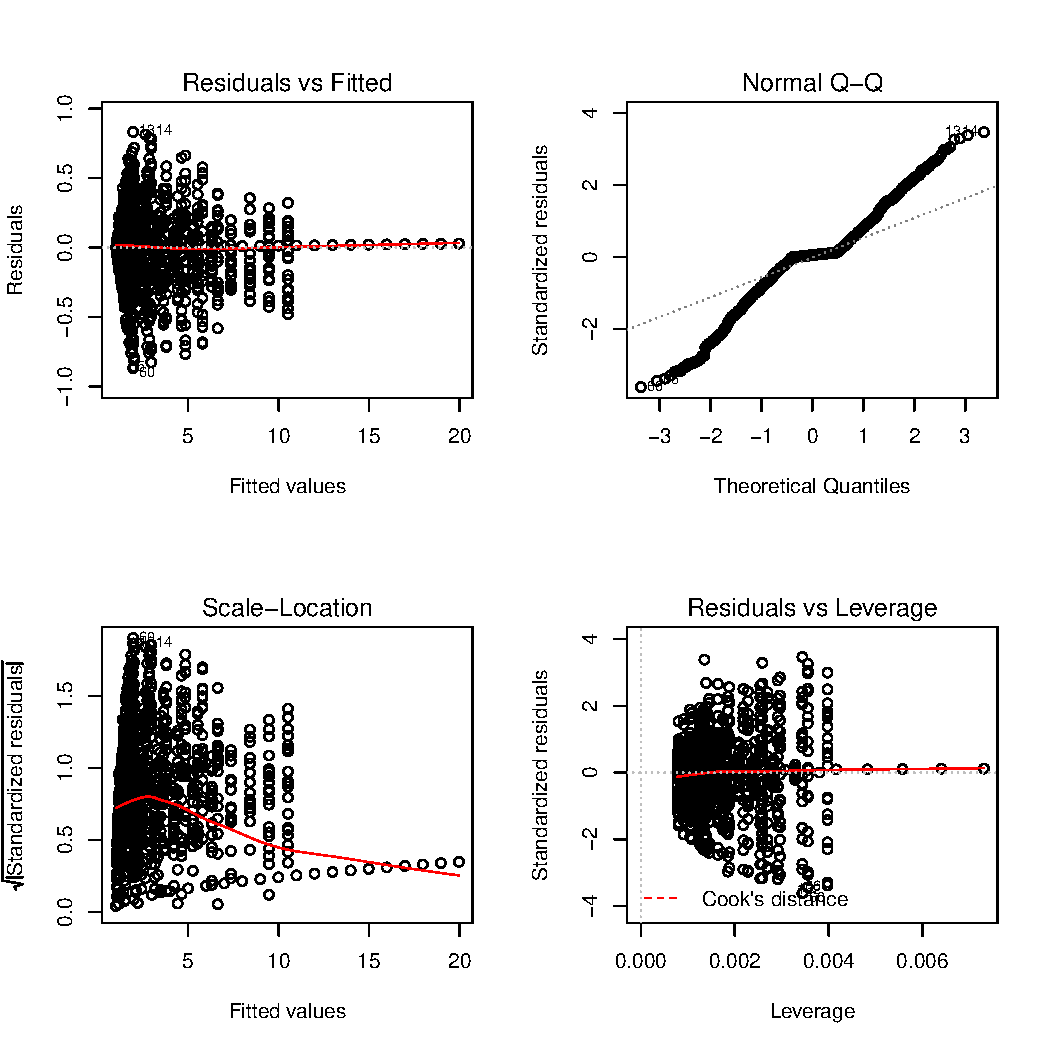
\includegraphics[width=\linewidth]{../../../Results/Simulation2/NicheAreaLmPlot_20.pdf}
    \caption{maxArea = 20 units}
  \end{subfigure}
  \caption{Model validation: Diagnostic plots of multivariate analysis of niche, area and species richness with full data set (a) and reduced data set (b)}
  \label{fig:Model validation multivariate 2}
\end{figure}\bigskip


\noindent Visual inspection of the residual results of the full dataset for migration/area/niche multivariate analysis showed non-linear, non-constant variance variance (Figure 7 (a)). The Q-Q plot deviates at lowest values. \bigskip

\noindent Visual inspection of the residual results of the full dataset for area/niche multivariate analysis showed fairly linear, non-constant variance, with variance greatest for higher values (Figure 8 (a)). The Q-Q plot deviates considerably from the line. \bigskip

\noindent Multivariate analysis results for the most reduced dataset showed that the combined effects of number of niches, island area and migration rate, gave an r-squared value of 0.999 (Table 3). The combined effects of niche and area gave an r-squared value of 0.998, indicating that migration rate had almost no effect on species richness at smaller island area. \bigskip

\noindent Visual inspection of the residual results of the reduced dataset for migration/area/niche multivariate analysis showed linear, non-constant variance (Figure 7 (b)). The Q-Q plot follows a relatively straight line. \bigskip 

\noindent Visual inspection of the residual results of the reduced dataset for area/niche multivariate analysis showed linear, non-constant variance (Figure 8 (b). The Q-Q plot deviates considerably from the line. 

\subsection{Simulation/Model Comparison}

\subsubsection{Outliers}

\begin{figure}[h!]
  \centering
  \begin{subfigure}[b]{0.4\linewidth}
    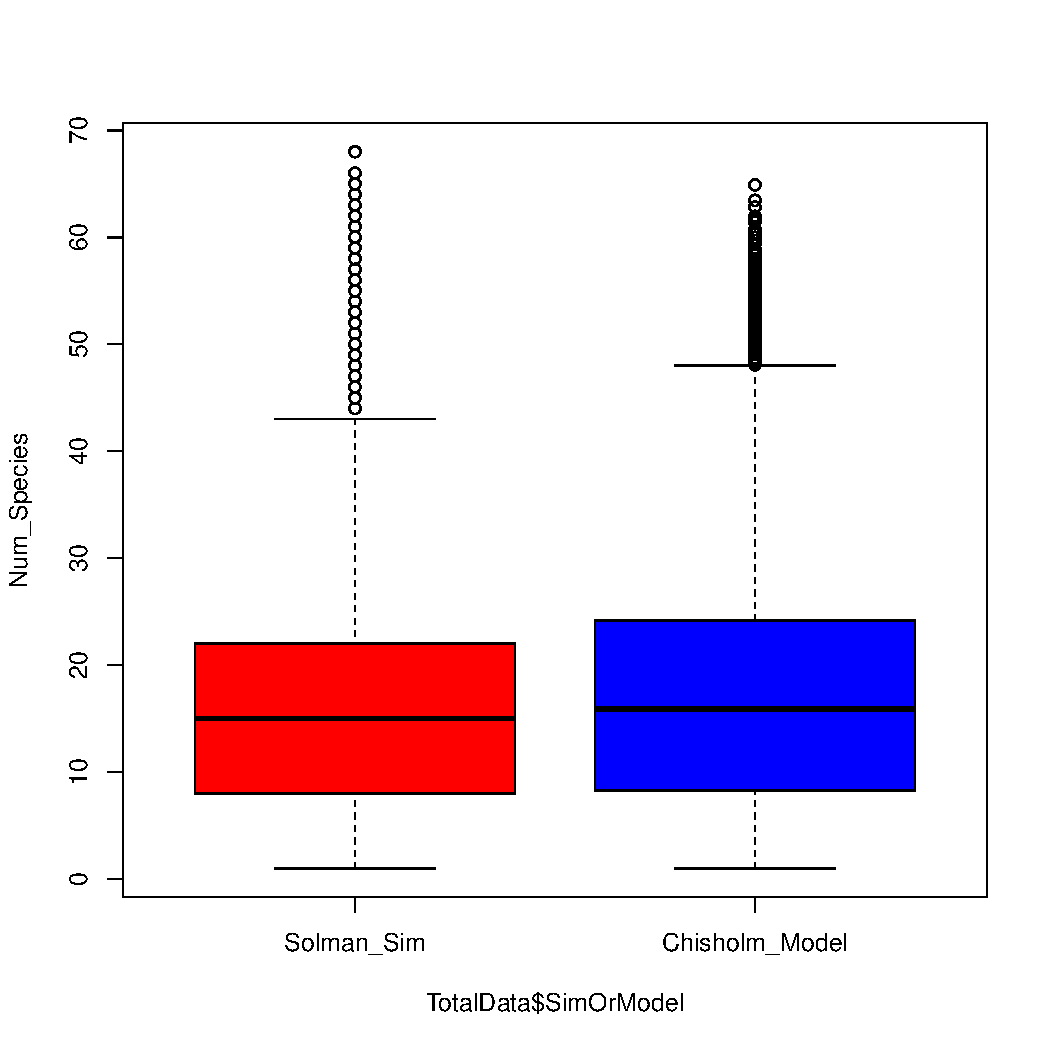
\includegraphics[width=\linewidth]{../../../Results/Simulation2/SolmanChisholmBoxplot_1.pdf}
    \caption{maxArea = 400 units}
  \end{subfigure}
  \begin{subfigure}[b]{0.4\linewidth}
    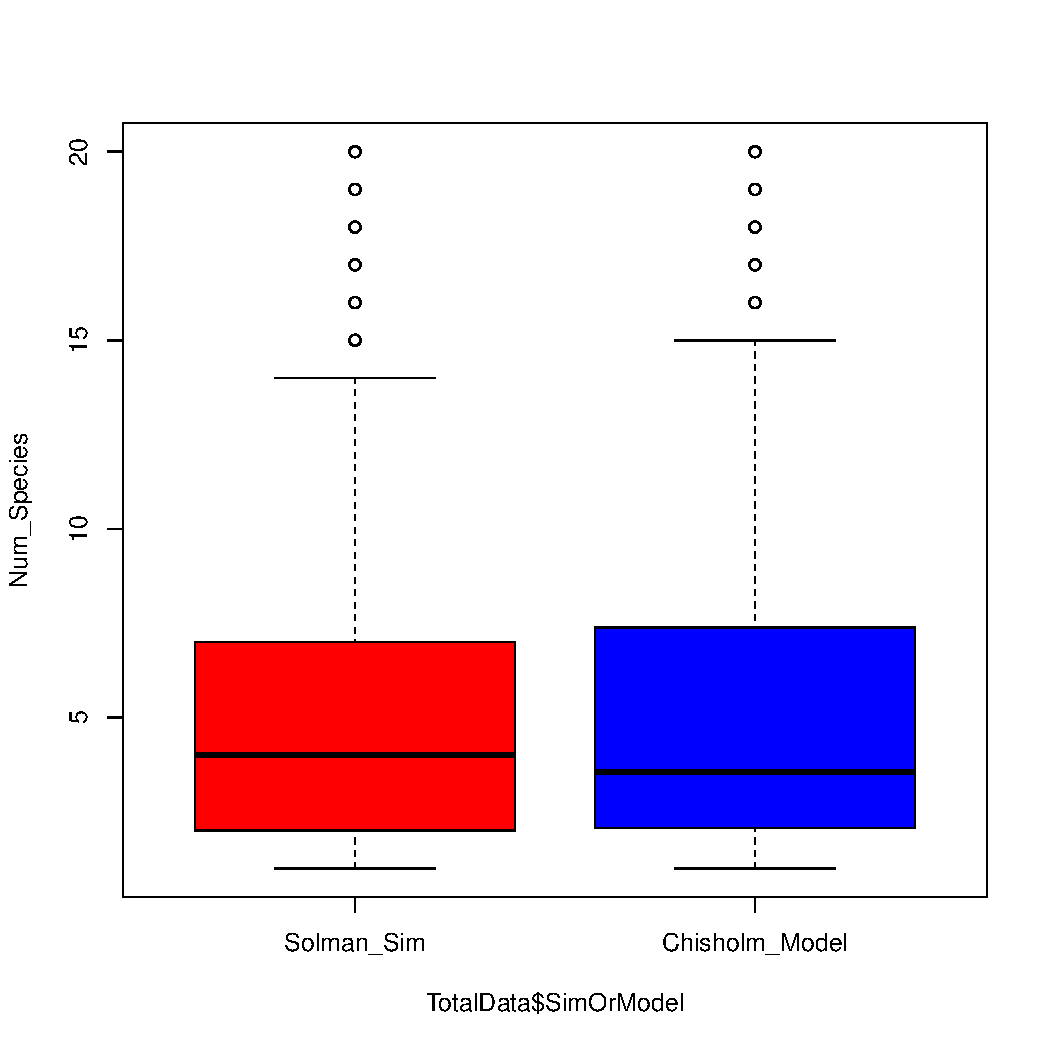
\includegraphics[width=\linewidth]{../../../Results/Simulation2/SolmanChisholmBoxplot_20.pdf}
    \caption{maxArea = 20 units}
  \end{subfigure}
  \caption{Boxplot of simulation and model estimation data for the full dataset (a) and area reduced dataset (b)}
  \label{fig:boxplots}
\end{figure}

\noindent Comparison of boxplots of simulated and model estimated species richnesses for the full dataset show outlying data points (Figure 9 (a)). On examining the simulation data, the plotted points represented 9658 islands that had species richness values $>$= 45. The model estimating data had 10600 islands with $>$= 50 species. As the number of islands present in both these outlier groups was so high, it was inappropriate to remove them from the data set as they represent a significant contribution to the overall mean. \bigskip

\noindent Boxplots of the reduced data also indicate outliers in both the simulation and model estimate datasets (Figure 9 (b)). 12000 islands in the simulation data set had species richness $>$= 15 and 10000 islands in the model estimation dataset had species richness $>$= 16. The outliers do not appear to be random deviates from the data, but represent a considerable proportion of the overall dataset and are not removed from this analysis.  

\subsubsection{Mean, range, variance, standard deviation and standard error}

\begin{table}[h!]
\caption{Mean, range, variance, SD and SE for simulation and model estimates}
\centering
\pgfplotstabletypeset[
    col sep=comma,
    ignore chars={"}, %get rid of quote marks around my text
    string type,
    every head row/.style={%
        before row={\hline
           % \multicolumn{2}{c}{incase you wanted a title above the column headers} & \\
        },
        after row=\hline
    },
    every last row/.style={after row=\hline},
    columns/mean/.style={column name=Mean, column type=c},
    columns/range/.style={column name=Range, column type=c},
    columns/variance/.style={column name=Variance, column type=c},
    columns/standarddeviation/.style={column name=StandardDeviation, column type=c},
    columns/standarderror/.style={column name=StandardError, column type=c},
    columns/maxArea/.style={column name=maxArea, column type=c},
    columns/ModelOrSim/.style={column name=ModelOrSim, column type=l},
    ]{../../../Results/Simulation2/StatsEdit.csv}
   \end{table}
    
\noindent For the full dataset, the mean number of species on simulated islands was 16.05 (SD 10.466, SE 0.012, range: 1-68) (Table 4).
The mean number of species estimated by the model was 17.60 (SD 11.79 , SE 0.01, range: 1-64.89). For the reduced island area dataset, the mean number of species on simulated islands was 5.49 (SD 4.99, SE 0.01, range: 1-20). The mean number of species estimated by the model was  5.59 (SD 5.12, SE 0.01, range: 1-20).

\subsubsection{Paired-sample t-Test}

\begin{table}[h!]
\caption{Paired-sample t-test for simulation data and model estimations}
\centering
\pgfplotstabletypeset[
    font={\small},
    %begin table=\begin{longtable},
    %end table=\end{longtable},
    col sep=comma,
    ignore chars={"}, %get rid of quote marks around my text
    string type,
    every head row/.style={%
        before row={\hline
           % \multicolumn{2}{c}{incase you wanted a title above the column headers} & \\
        },
        after row=\hline
    },
    every last row/.style={after row=\hline},
    columns/mean/.style={column name=MeanDifference, column type=c},
    columns/tvalue/.style={column name=tValue, column type=c},
    columns/pvalue/.style={column name=pValue, column type=l},
    columns/df/.style={column name=DF, column type=c},
    columns/conflow/.style={column name=ConfLow, column type=c},
    columns/confhigh/.style={column name=ConfHigh, column type=c},
    columns/method/.style={column name=Method, column type=l},
    columns/alternative/.style={column name=Alternative, column type=l},
    columns/maxArea/.style={column name=maxArea, column type=c},
    ]{../../../Results/Simulation2/pairedtMaxMin.csv}
   \end{table}\bigskip
   
\noindent The mean difference between simulation results and model estimations for the full dataset was -1.55, with a t-value of -155.01 and a p-value of $<$ 0.001 (DF 799999, CI low -1.55, CI high -1.54). The mean difference between simulation results and model estimations for the most reduced dataset were -0.1, with a t-value of -64.1 and a p-value of $<$ 0.001 (DF 131999, CI low -0.1, CI high -0.09). In both cases, p $<$ 0.001, therefore we reject the null hypothesis that there is no difference in the simulated and model estimated datasets. However, the mean differences are small and for the most reduced dataset represent species $<$ 1, a logical impossibility.  

\subsubsection{Non-Linear Least Squares Fitting}      
   
\begin{table}[h!]
\caption{NLLS fitting of Chisholm model to simulation data, parameter statistics for 3 out of 400 fits}
\centering
\pgfplotstabletypeset[
    col sep=comma,
    ignore chars={"}, %get rid of quote marks around my text
    string type,
    every head row/.style={%
        before row={\hline
           % \multicolumn{2}{c}{incase you wanted a title above the column headers} & \\
        },
        after row=\hline
    },
    every last row/.style={after row=\hline},
    columns/terms/.style={column name=Terms, column type=c},
    columns/estimate/.style={column name=Estimate, column type=c},
    columns/standarderror/.style={column name=StandardError, column type=c},
    columns/statistic/.style={column name=Statistic, column type=c},
    columns/pvalue/.style={column name=pValue, column type=c},
    columns/rsquared/.style={column name=rSquared, column type=c},
    columns/migrationrate/.style={column name=MigrationRate, column type=c},
    columns/niches/.style={column name=Niches, column type=c},
     columns/numislands/.style={column name=NumIslands, column type=c},
    ]{../../../Results/Simulation2/NLLS/SumResults.csv}
   \end{table}\bigskip
   
\noindent NLLS fitting was used to fit the \textit{chisholm\_function} to 400 subsets of island data (unique migration rate + unique niche number). This was to test whether, through NLLS fitting, the model could produce robust parameter estimates of the known migration and niche values for each dataset. 395 out of 400 model fits had a r-squared value of $>$ 0.9. The remaining five fits had r-squared values of between 0.595 and 0.897. This indicates that for most datasets the model fit the data well. \bigskip

\noindent Table 6 shows parameter estimates and statistical values for NLLS fitting 1, 190 and 400. Fits 200 and 400 show high r-squared values with significant niche and migration parameters ( p $<$ 0.001). Migration rate is statistically insignificant for the 1 niche dataset. \textit{Theta} estimates for all three fits are much higher than realistically possible. \textit{m0} estimations are within the range of true values where (\textit{m = m0/sqrt(area)}). Niche (\textit{K}) estimations are also fairly accurate. Visual inspection of the direct model estimations and NLLS fitting reveal both were successful in predicting species richness on the simulated islands (Figure 10).

\begin{figure}[h!]
  \centering
  \begin{subfigure}[b]{0.3\linewidth}
    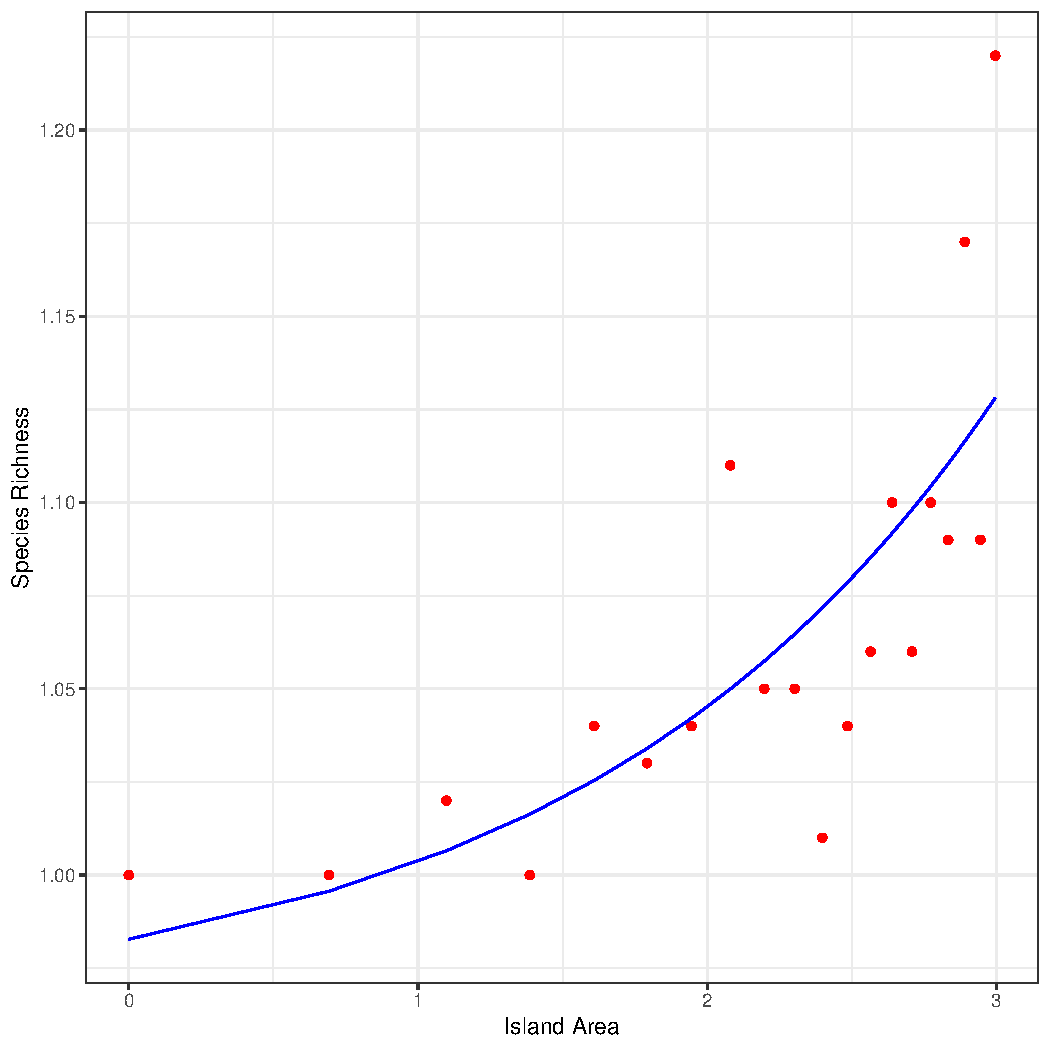
\includegraphics[width=\linewidth]{../../../Results/Simulation2/NLLS/NLLSfits_1.pdf}
     \caption{NLLS Plot 1}
  \end{subfigure}
  \begin{subfigure}[b]{0.3\linewidth}
    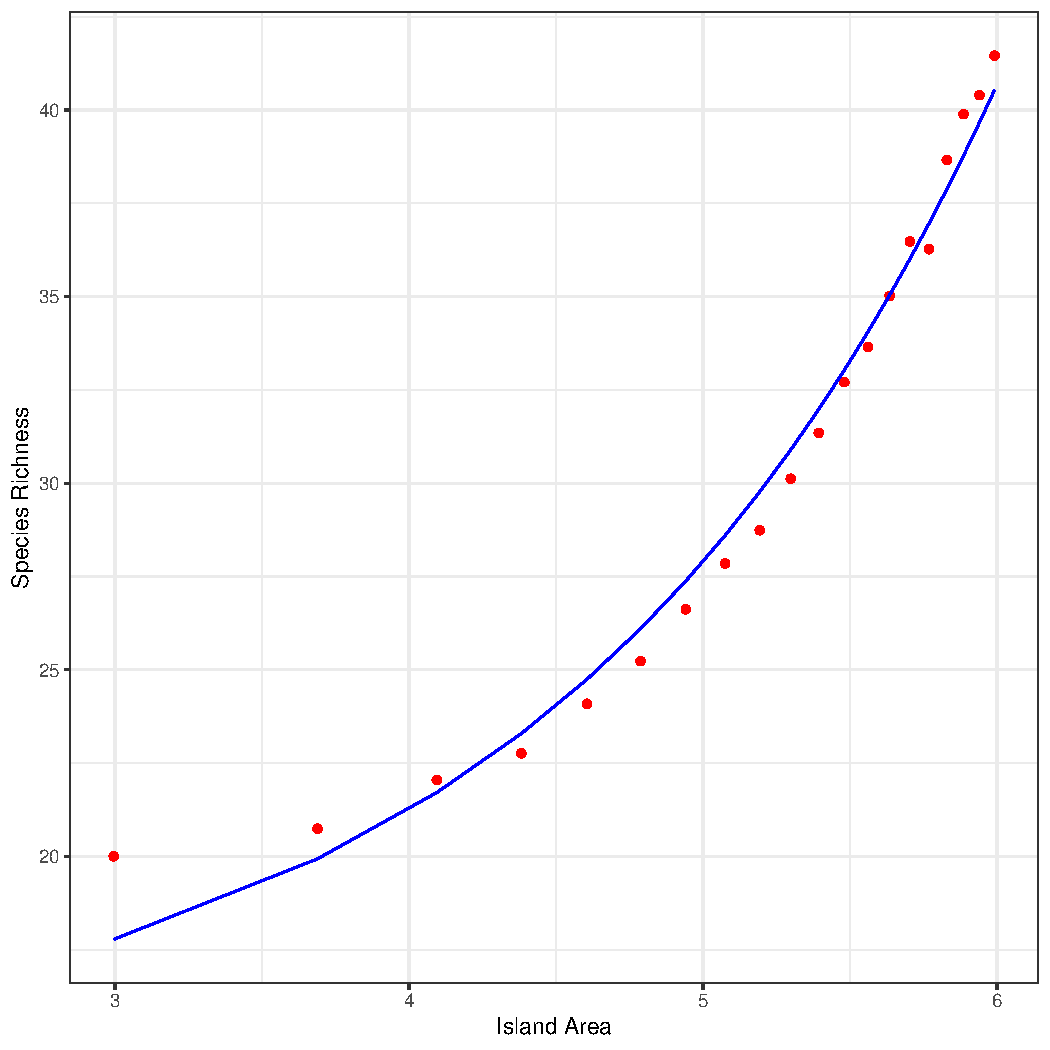
\includegraphics[width=\linewidth]{../../../Results/Simulation2/NLLS/NLLSfits_200.pdf}
    \caption{NLLS Plot 200}
  \end{subfigure}
  \begin{subfigure}[b]{0.3\linewidth}
    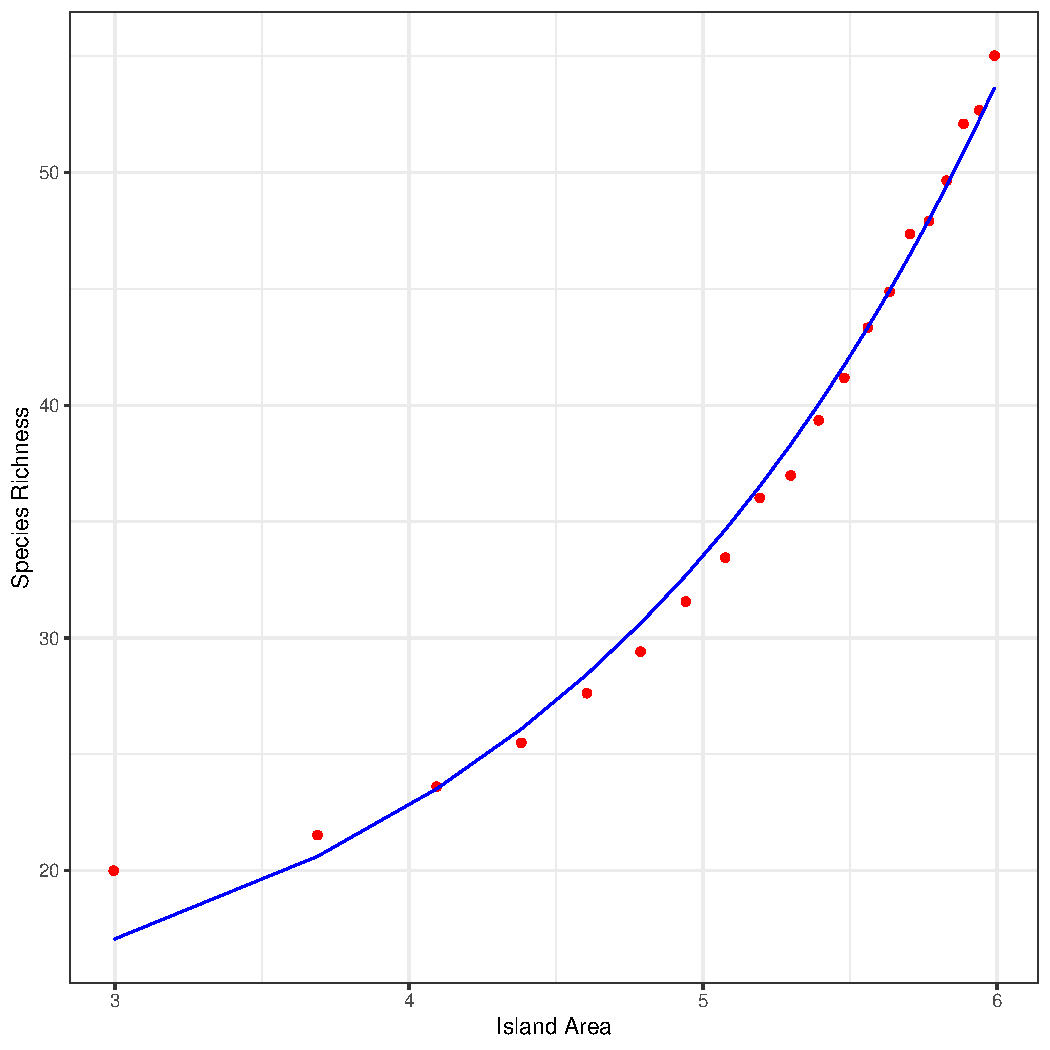
\includegraphics[width=\linewidth]{../../../Results/Simulation2/NLLS/NLLSfits_400.pdf}
    \caption{NLLS Plot 400}
  \end{subfigure}
  \begin{subfigure}[b]{0.5\linewidth}
    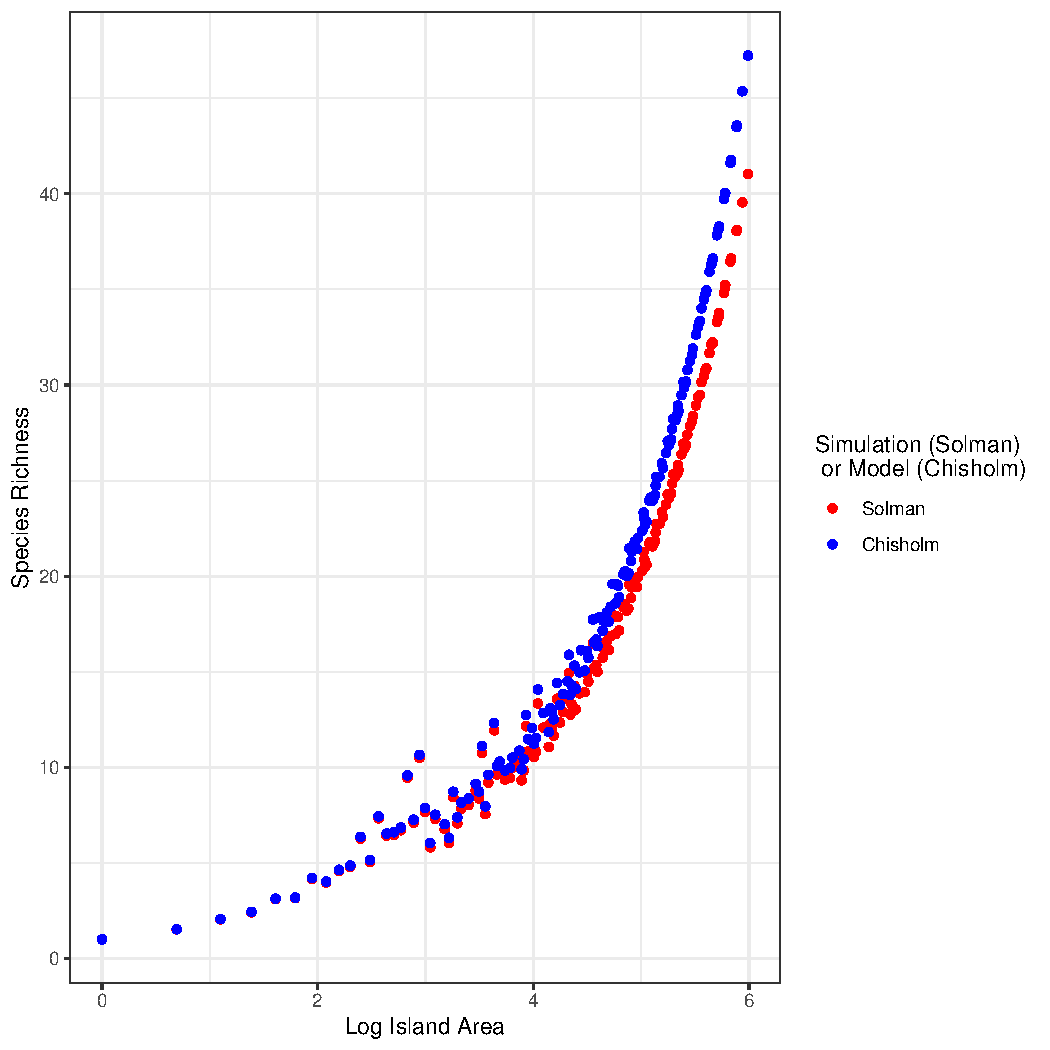
\includegraphics[width=\linewidth]{../../../Results/Simulation2/MeanResultsPlot.pdf}
    \caption{Direct estimations of species richness}
  \end{subfigure}
  \caption{Comparison of model fitting directly using the \textit{chisholm\_function} on mean dataset (d), and using NLLS fitting for subsets of data (a, b, c)}
  \label{fig:fitting}
\end{figure}

  


\end{document}